%! Author = angel
%! Date = 1/28/25

% Preamble
\documentclass[11pt]{article}

% Packages
\usepackage{amsmath,amssymb,amsthm}
\usepackage[letterpaper,margin=0.75in]{geometry}
\usepackage{pgfplots}
\usepackage{tikz}
\usepackage{xcolor}
\usepackage{fancyhdr}
\pgfplotsset{compat=1.18}
\usepackage{tikz-cd}

\usetikzlibrary{decorations.markings, arrows.meta}
% Document
\tikzset{
    marrow/.style={decoration={markings,mark=at position 0.5 with {\arrow{#1}}}, postaction=decorate}
}


\begin{document}
    \noindent \textbf{Chapter 17 - Waves II}
    \\ \noindent \newline Sound waves are considered longitudinal waves modeled by the equation:
    \begin{equation}
        s(x,t) = s_m\cos(kx - \omega t + \phi) \tag{sound equation}
    \end{equation}


    \noindent In 2D space, the travel of sound waves can be visualized by circles
    emitting out of the source.
    These \textbf{wavefronts} show where the oscillations have the same value.
    We can show the direction of the waves travel using \textbf{rays.}

    \\ \hfill
    \begin{minipage}[b]{0.3\textwidth}
        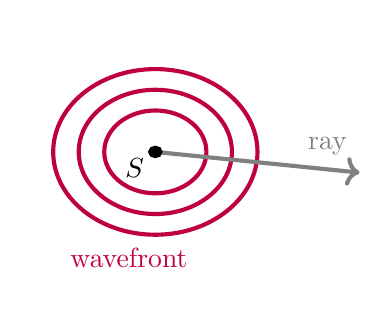
\begin{tikzpicture}
            \tikzstyle{every path}=[line width=1.5pt]
            \begin{axis}[
                ytick=\empty,
                xtick=\empty,
                samples=1000,
                axis line style={draw=none},
                enlargelimits=false,
                height=5cm,
                xmin=-1, xmax=12,
                ymin=-1, ymax=12
            ]
                \draw[draw=purple] (axis cs: 4, 6) circle [radius=2];
                \draw[draw=purple] (axis cs: 4, 6) circle [radius=3];
                \draw[draw=purple] (axis cs: 4, 6) circle [radius=4] node[midway, above= 0.5cm, right=0.4cm,purple] {wavefront};
                \draw[->,gray] (4,6) -- (12,5) node[midway, above=0.2cm, right=0.5cm] {ray};
                \draw[fill=black] (4,6) circle (0.2) node[below=0.2cm, left] {$S$};
            \end{axis}
        \end{tikzpicture}
    \end{minipage}
    \hfill
    \begin{minipage}[b] {0.6\textwidth}
        \begin{equation}
            v = \sqrt{\frac{B}{\rho}} = 343 \text{ m/s} \tag{speed of sound in air}\label{eq:soundSpeed}
        \end{equation}
        As sound waves pass through the air, areas of compression and expansion form,
        in which we can find the speed by finding $B$, the rate of change of pressure over a volume (bulk modulus),
        and $\rho$ the density of the medium.
    \end{minipage}

    \noindent \\ Since the speed of the wave is determined by its medium, not frequency,
    we can find the wavelength using the same formula from CH16 ($\lambda = \frac{v}{f} = \frac{343}{f}$).
    We can find the \textbf{change in pressure} (Pa) caused by sound waves:
    \begin{equation}
       \Delta \rho = \Delta \rho_m \sin(kx - \omega t) \tag{pressure}
    \end{equation}
    Where the pressure amplitude (Pa) given power and displacement is:
    \begin{equation}
     \Delta \rho_m = (v \rho \omega)s_m \tag{pressure amplitude}
    \end{equation}

    \noindent \\ Moving away from the source, the intensity of sound waves gradually decreases.
    \textbf{Intensity} (W/\text{m}$^{2}$) is the average power a sound wave carries per unit area:

    \begin{equation}
        I = \frac{1}{2} \rho v \omega^2 s_{m}^2 \tag{intensity}\label{eq:intensity}
    \end{equation}

    \noindent We can find the intensity at any distance $r$ away from the source using the formula:
    \begin{equation}
        I = \frac{P_s}{4 \pi r^2} \tag{intensity at distance r}
    \end{equation}

    \noindent Note that intensity is proportional to the pressure squared
    ($I \propto \rho^2$).
    However, we measure \textbf{sound level} in decibels (dB) using a logarithmic scale
    where $I_0$ is the standard reference intensity ( $10^{-12}$ W/m^2).

    \begin{equation}
        \beta = (10 \text{dB}) \log \frac{I}{I_0} \tag{sound level}
    \end{equation}

    \noindent Sources of sound waves are not always stationary,
    in fact their velocity changes their perceived frequency.

     \hfill
    \begin{minipage}[b]{0.25\textwidth}
        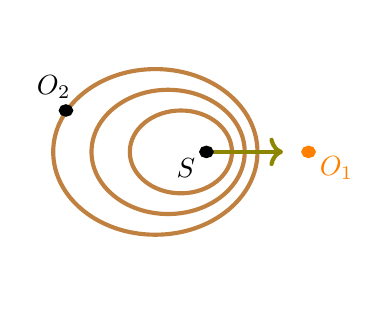
\begin{tikzpicture}
            \tikzstyle{every path}=[line width=1.5pt]
            \begin{axis}[
                ytick=\empty,
                xtick=\empty,
                samples=1000,
                axis line style={draw=none},
                enlargelimits=false,
                height=5cm,
                xmin=-1, xmax=12,
                ymin=-1, ymax=12
            ]
                \draw[draw=brown] (axis cs: 5, 6) circle [radius=2];
                \draw[draw=brown] (axis cs: 4.5, 6) circle [radius=3];
                \draw[draw=brown] (axis cs: 4, 6) circle [radius=4];
                \draw[->,olive] (6,6) -- (9,6);
                \draw[fill=black] (6,6) circle (0.2) node[below=0.2cm, left] {$S$};
                \draw[orange, fill=orange] (10,6) circle (0.2) node[orange, below=0.2cm, right] {$O_1$};
                \draw[black, fill=black] (0.5,8) circle (0.2) node[black, above=0.3cm, left=-0.2cm] {$O_2$};
            \end{axis}
        \end{tikzpicture}
    \end{minipage}
    \hfill
    \begin{minipage}[b] {0.7\textwidth}
        Where $v_o$ is the velocity of the observer, and $v_s$ is the velocity of the source.
        Frequency changes:
        \begin{equation}
            f' = f \frac{v \pm v_o}{v \mp v_s }  \tag{Doppler Effect}\label{doppler}
        \end{equation}

        The wavefronts show that the frequency increases as $\Delta x$ decreases, and vice versa.
    \end{minipage}

    \noindent \\
    With this in mind, the top equation is addition if $v_0$ is going towards the source,
    while the bottom is negative if $v_s$ is moving towards the observer.
    The signs switch if they go in the other direction (going away).

   \newpage
    \noindent \textbf{Chapter 17 - Waves II}
    \noindent \\ \\Multiple sound waves can interfere with each other creating both constructive
    and destructive interference.

    \begin{center}
        \makebox[\textwidth]{%
            \begin{minipage}{0.2\textwidth} % Adjust width for graphs
                \centering
                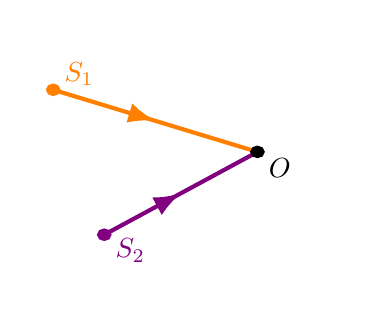
\begin{tikzpicture}
                    \tikzstyle{every path}=[line width=1.5pt]
                    \begin{axis}[
                        ytick=\empty,
                        xtick=\empty,
                        samples=1000,
                        axis line style={draw=none},
                        enlargelimits=false,
                        height=5cm,
                        xmin=-1, xmax=12,
                        ymin=-1, ymax=12
                    ]
                        \draw[orange, fill=orange] (0,9) circle (0.2) node[orange, above=0.2cm, right] {$S_1$};
                        \draw[-,orange, marrow=Latex] (0,9) -- (8,6);
                        \draw[violet, fill=violet] (2,2) circle (0.2) node[violet, below=0.2cm, right] {$S_2$};
                        \draw[-,violet, marrow=Latex] (2,2) -- (8,6);
                        \draw[fill=black] (8,6) circle (0.2) node[below=0.2cm, right] {$O$};
                    \end{axis}
                \end{tikzpicture}
            \end{minipage}
            \hfill
            \parbox{0.73\textwidth}{%
                \noindent Remembering that the resultant wave of two waves with the same wavelength is
                $2y_{m}\cos(\frac{\phi}{2}) \sin(kx - \omega t + \frac{\phi}{2})$,
                we can correspond the phase offset ($\frac{\phi}{2}$)
                to the path length difference ($\Delta L$).
                This gives us:
                \begin{equation}
                    \phi = \frac{\Delta L}{\lambda} 2 \pi \tag{phase difference}
                \end{equation}
            }
        }

        \makebox[\textwidth]{%
            \begin{minipage}{0.2\textwidth}
                \centering
                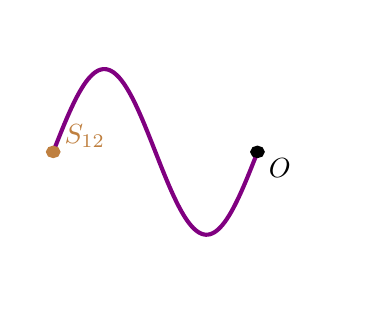
\begin{tikzpicture}
                    \tikzstyle{every path}=[line width=1.5pt]
                    \begin{axis}[
                        ytick=\empty,
                        xtick=\empty,
                        samples=1000,
                        axis line style={draw=none},
                        enlargelimits=false,
                        height=5cm,
                        xmin=-1, xmax=12,
                        ymin=-1, ymax=12
                    ]
                        \addplot[domain=0:8, samples=100, thick, violet]
                        ({x}, {6 + 4*sin(deg(3.14*x/4))});
                        \draw[brown, fill=brown] (0,6) circle (0.2) node[brown, above=0.2cm, right] {$S_{12}$};
                        \draw[fill=black] (8,6) circle (0.2) node[below=0.2cm, right] {$O$};
                    \end{axis}
                \end{tikzpicture}
            \end{minipage}
            \hfill
            \parbox{0.73\textwidth}{%
                \noindent With this equation we can check if it's \textbf{fully constructive interference}
                (creating a larger wave) when
                $\phi$ is an integer multiple of $\pi$:
                \begin{equation}
                    \phi = m(2\pi) \text{ or } \frac{\Delta L}{\lambda} = 0,1,2,... \tag{fully constructive}
                \end{equation}
            }
        }

        \makebox[\textwidth]{%
            \begin{minipage}{0.2\textwidth}
                \centering
                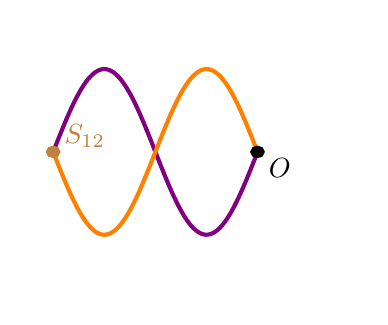
\begin{tikzpicture}
                    \tikzstyle{every path}=[line width=1.5pt]
                    \begin{axis}[
                        ytick=\empty,
                        xtick=\empty,
                        samples=1000,
                        axis line style={draw=none},
                        enlargelimits=false,
                        height=5cm,
                        xmin=-1, xmax=12,
                        ymin=-1, ymax=12
                    ]
                        \addplot[domain=0:8, samples=100, thick, violet]
                        ({x}, {6 + 4*sin(deg(3.14*x/4))});
                        \addplot[domain=0:8, samples=100, thick, orange]
                        ({x}, {6 - 4*sin(deg(3.14*x/4))});
                        \draw[brown, fill=brown] (0,6) circle (0.2) node[brown, above=0.2cm, right] {$S_{12}$};
                        \draw[fill=black] (8,6) circle (0.2) node[below=0.2cm, right] {$O$};
                    \end{axis}
                \end{tikzpicture}
            \end{minipage}
            \hfill
            \parbox{0.73\textwidth}{%
                \noindent \textbf{Fully destructive interference}
                (where the two are out phases creating a smaller wave)
                occurs when $\phi$ is an odd multiple of $\pi$:
                \begin{equation}
                    \phi = (2m+1)\pi \text{ or } \frac{\Delta L}{\lambda} = 0.5,1.5,2.5,... \tag{fully destructive}
                \end{equation}
                \noindent where m is an integer (0,1,2,...)
            }
        }
    \end{center}

    \noindent When two different frequencies are played together, either interfering constructively (getting louder) or
    destructively (getting quieter), the difference between the frequencies create \textbf{beats:}
    \begin{equation}
        f_{beat} = \left |f_1 - f_2 \tag{beat frequency} \right|
    \end{equation}

    \noindent Similar to strings, Sound can create standing waves in a pipe.
    Now we can find the resonant frequencies:
    \begin{minipage}[b]{0.25\textwidth}
        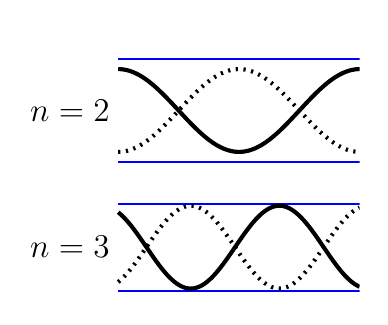
\begin{tikzpicture}
            \tikzstyle{every path}=[line width=1.5pt]
            \begin{axis}[
                ytick=\empty,
                xtick=\empty,
                samples=1000,
                axis line style={draw=none},
                enlargelimits=false,
                height=5cm,
                xmin=-1, xmax=10,
                ymin=-1, ymax=12
            ]
                \draw[thick,blue] (2,10.5) -- (10,10.5);
                \draw[thick,blue] (2,5.5) -- (10,5.5);
                \addplot[domain=2:10, samples=100, thick, black]
                ({x}, {8 + 2*sin(deg(3.14*x/4))});
                \addplot[dotted,domain=2:10, samples=100, thick, black]
                ({x}, {8 - 2*sin(deg(3.14*x/4))});

                \draw[thick,blue] (2,3.5) -- (10,3.5);
                \draw[thick,blue] (2,-0.7) -- (10,-0.7);
                \addplot[domain=2:10, samples=100, thick, black]
                ({x}, {1.4 + 2*sin(deg(4.28*x/4))});
                \addplot[dotted,domain=2:10, samples=100, thick, black]
                ({x}, {1.4 - 2*sin(deg(4.28*x/4))});

                \node at (0.4, 8) {\large $n = 2$};
                \node at (0.4, 1.4) {\large $n = 3$};
            \end{axis}
        \end{tikzpicture}
    \end{minipage}
    \hspace{0.001\textwidth} % Adjust horizontal spacing
    \begin{minipage}[b]{0.25\textwidth}
        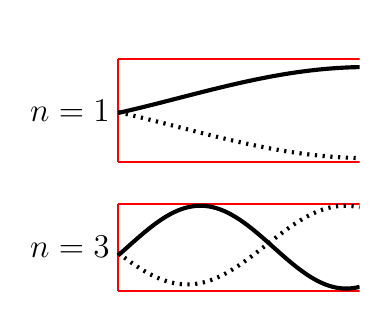
\begin{tikzpicture}
            \tikzstyle{every path}=[line width=1.5pt]
            \begin{axis}[
                ytick=\empty,
                xtick=\empty,
                samples=1000,
                axis line style={draw=none},
                enlargelimits=false,
                height=5cm,
                xmin=-1, xmax=10,
                ymin=-1, ymax=12
            ]
                \draw[thick,red] (2,10.5) -- (10,10.5);
                \draw[thick,red] (2,5.5) -- (10,5.5);
                \draw[thick,red] (2,10.5) -- (2,5.5);
                \addplot[domain=2:10, samples=100, thick, black]
                ({x}, {8.6 + 1.5*sin(deg(x/4 -1))});
                \addplot[dotted,domain=2:10, samples=100, thick, black]
                ({x}, {7.2 - 1.5*sin(deg(x/4 - 1))});

                \draw[thick,red] (2,3.5) -- (10,3.5);
                \draw[thick,red] (2,-0.7) -- (10,-0.7);
                \draw[thick,red] (2,-0.7) -- (2,3.5);
                \addplot[domain=2:10, samples=100, thick, black]
                ({x}, {1.4 + 2*sin(deg(2.6*x/4-1.5))});
                \addplot[dotted,domain=2:10, samples=100, thick, black]
                ({x}, {1.5 - 1.9*sin(deg(2.4*x/4-1))});
                \node at (0.4, 8) {\large $n = 1$};
                \node at (0.4, 1.4) {\large $n = 3$};
            \end{axis}
        \end{tikzpicture}
    \end{minipage}
    \hspace{0.01\textwidth} % Adjust horizontal spacing
    \begin{minipage}[b]{0.46\textwidth}
\vspace{0.3cm}
        In a pipe with \textbf{both ends open} (blue), the ends of the pipe will always be antinodes.
        The pipe will work with \textbf{any harmonic number:}
        \begin{equation}
            \lambda = \frac{2L}{n} \tag{$\lambda$}
        \end{equation}
        \begin{equation}
            f = \frac{nv}{2L} \tag{resonance}
        \end{equation}
    \end{minipage}

    \vspace{0.3cm}
    \noindent In the pipe with \textbf{one end closed} (red),
    the closed side will be a node, and the open end is an antinode.
    However the \textbf{harmonic number must be an odd integer.}
    \begin{equation}
        \lambda = \frac{4L}{n}  \tag{\lambda}
    \end{equation}
    \begin{equation}
        f = \frac{nv}{4L} \tag{resonance}
    \end{equation}
\end{document}

